\documentclass[paper=a4, oneside, fontsize=11pt,
parskip=full]{scrartcl}

\usepackage{paralist}


\usepackage[T1]{fontenc}
\usepackage{lmodern}
\usepackage[english]{babel}
\usepackage{blindtext}
\usepackage{graphicx}

% for a reduced line spacing in list environments
\usepackage{paralist}
\usepackage{hyperref}

\usepackage{array}
\usepackage{booktabs}
\usepackage{listing}


\newcommand{\head}[1]{\textbf{#1}}

\title{ICM20948 : Getting Started}
\author{M.B.}
\date{08.08.2025}

\begin{document}
\noindent
\maketitle
\tableofcontents
	
\section{About the ICM20948}	

The ICM20948 chip is a 9-axis MEMS motion-tracking device providing:

\begin{compactitem}
	\item a 3 axis accelerometer
	\item a 3 axis gyroscope
	\item a 3 axis compass
\end{compactitem}



The datasheet can be found here:

\url{https://invensense.tdk.com/download-pdf/icm-20948-datasheet} \\

Additional information about how to connect the sensor to a Raspberry Pi can be found here: \url{https://cdn-learn.adafruit.com/downloads/pdf/adafruit-tdk-invensense-icm-20948-9-dof-imu.pdf}

According to this document the ICM20948 (communication via I2C) must be connected like this:

\begin{table}[h]
	\centering
	\begin{tabular}{ll}
		\head{ICM20948 connector} & \head{Raspberry Pi pin} \\
		\hline
		Vin (red wire) & Pin\#1 \\
		GND (black wire) & Pin\#6 \\
		SCL (yellow wire) & Pin\#5 \\
		SDA (blue wire) & Pin\#3 \\
		\hline
	\end{tabular}

\end{table}

Images of the ICM20948 and its I2C connection are shown here:

\begin{figure}[h]
	\centering
	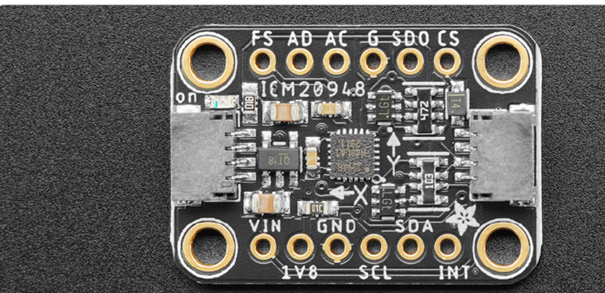
\includegraphics[width=6cm]{images/ICM20948.png}
	\caption{breakout board / ICM20948}
\end{figure}	

\begin{figure}[h]
	\centering
	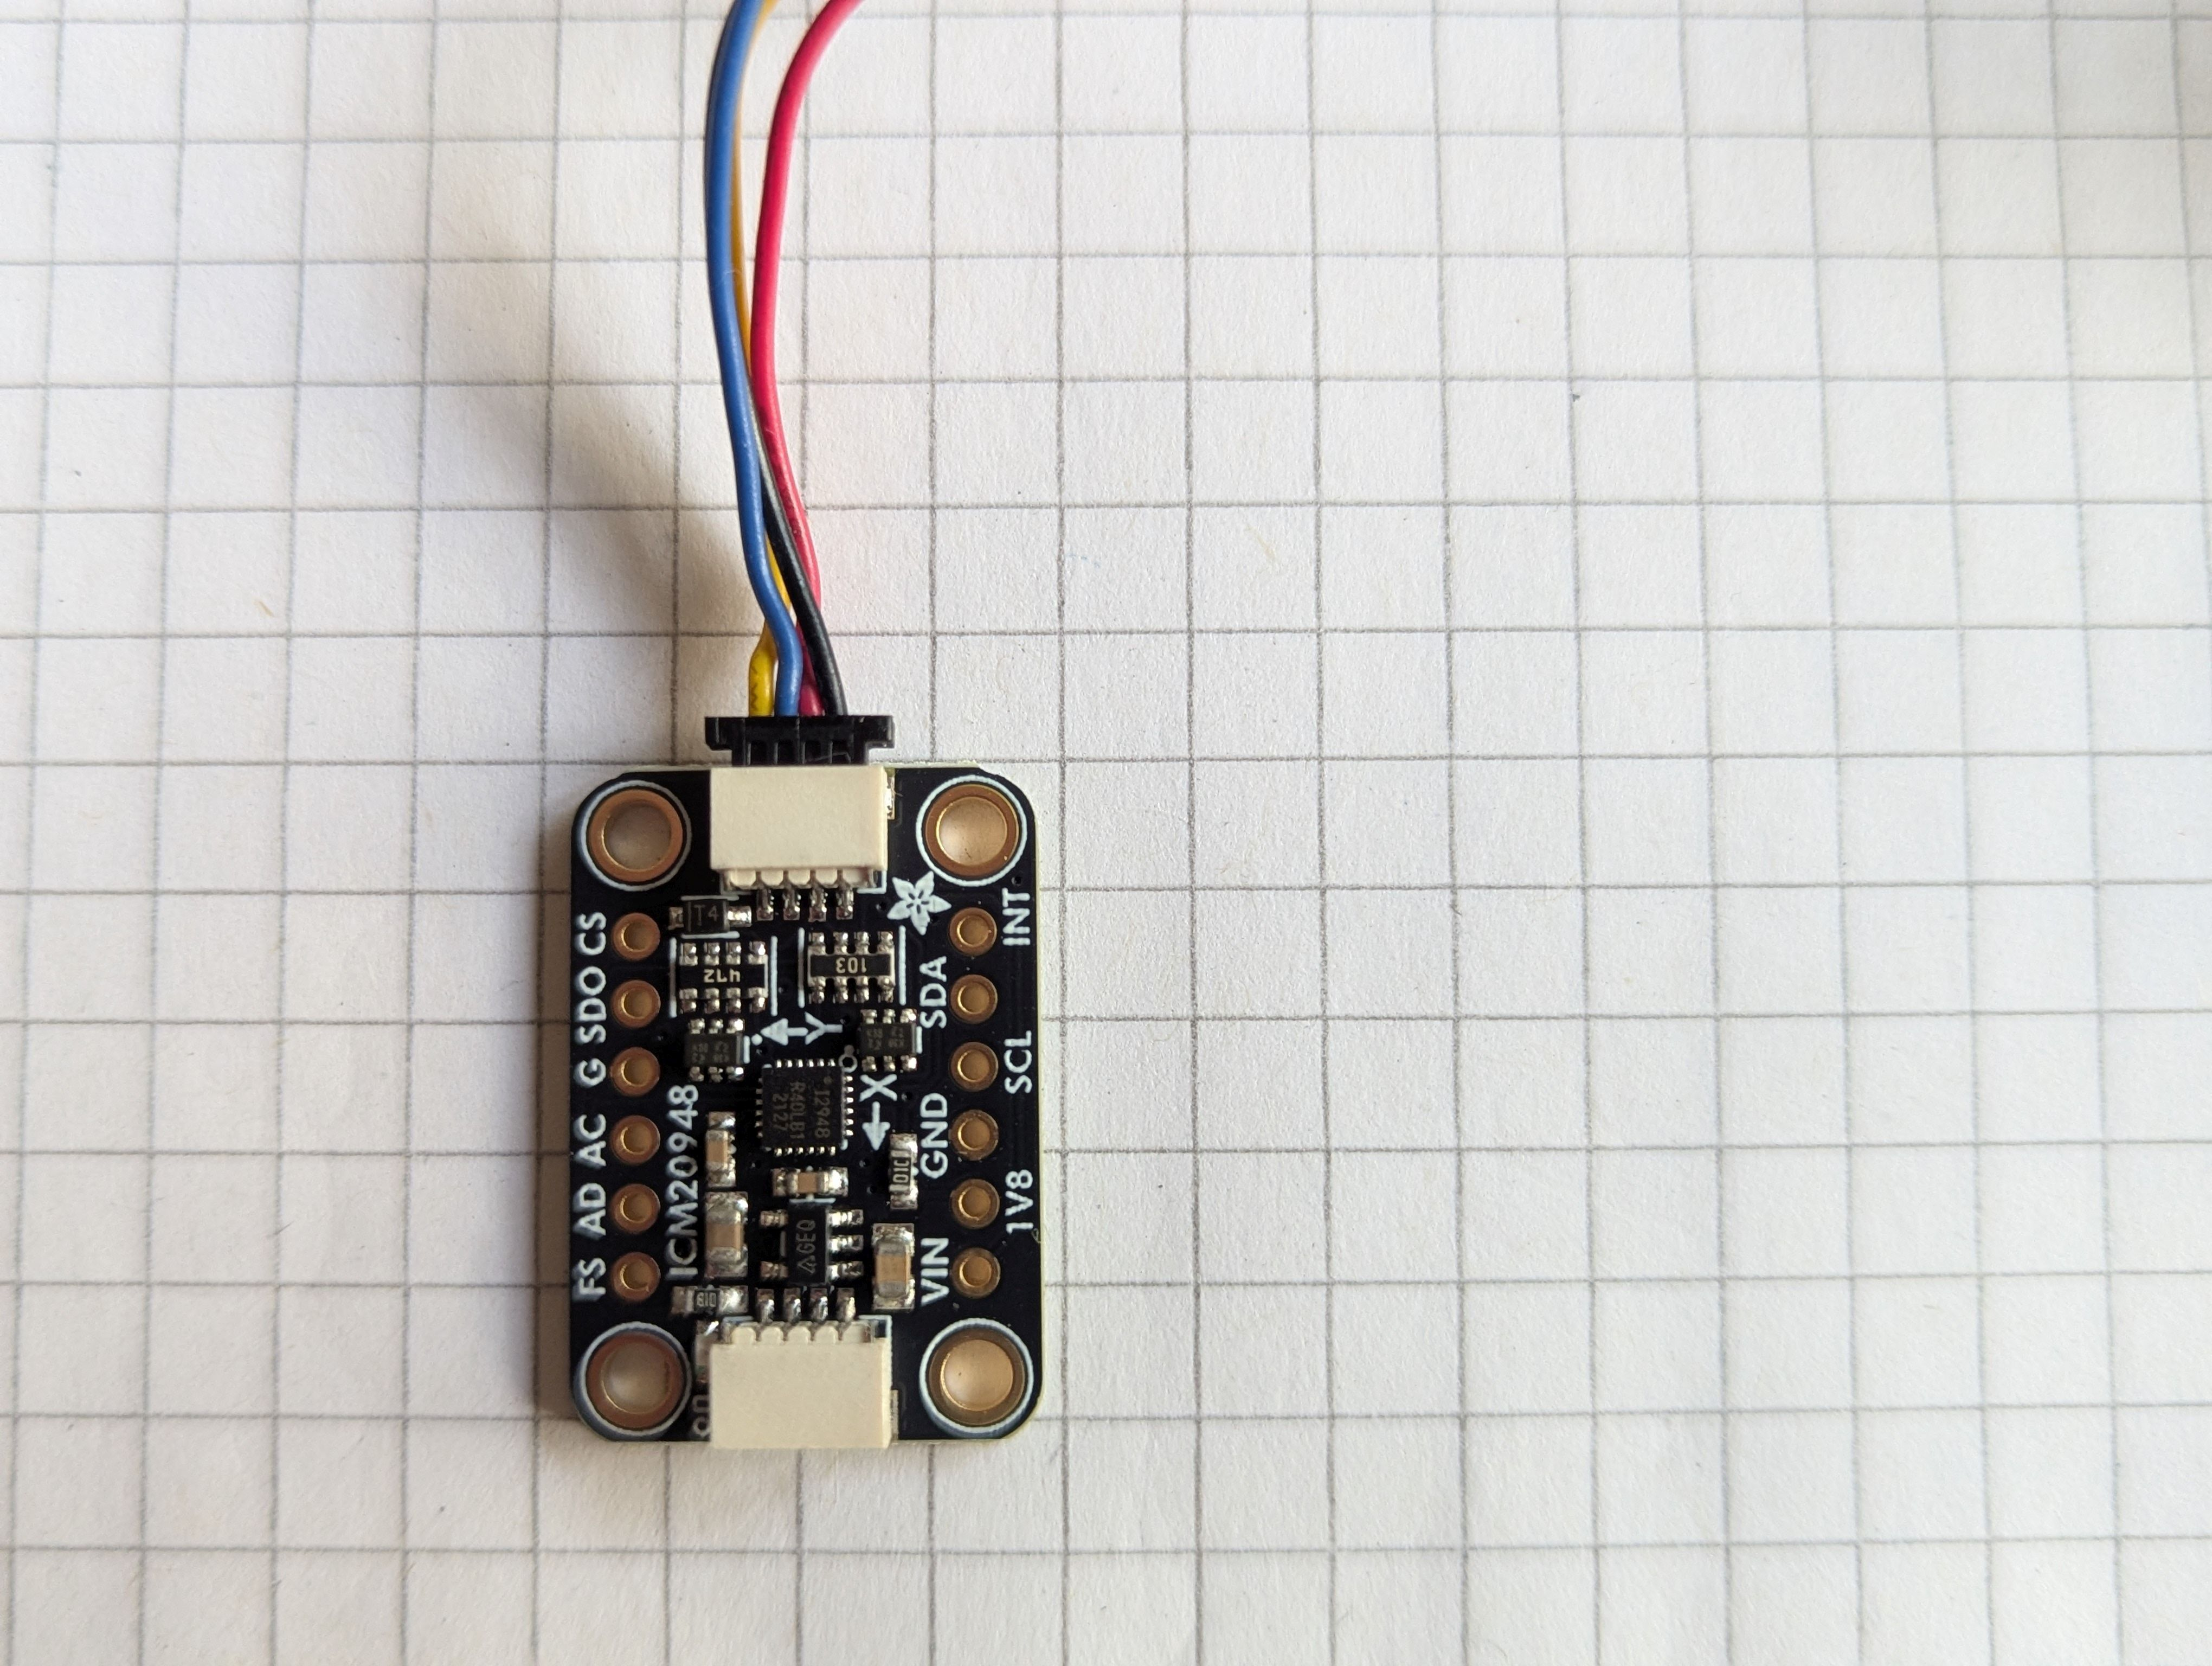
\includegraphics[width=6cm]{images/ICM20948.jpg}
	\caption{ICM20948 and its connections}
\end{figure}	

And here is a resource from the internet showing the Pins available on a Raspberry Pi 3/4.

\begin{figure}[h]
	\centering
	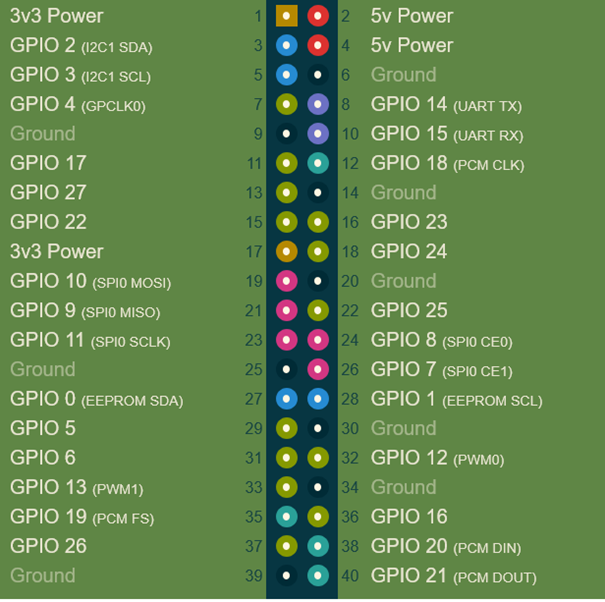
\includegraphics[width=6cm]{images/gpio_pins_rpi3.png}
	\caption{GPIO pins / Raspberry Pi 3}
\end{figure}	
	

Accessing the ICM20948 is done via I2C. So some preliminary tests should give us enough confidence that communication via I2C does work in principle. More advanced interactions with the ICM20948 will usually be accomplished  via Python programs.


A very readable book on how to interface with the Raspberry Pi is

\texttt{Raspberry PI, interfacing to the real world with embedded Linux}; autor: Derek Molloy.

This book has a chapter \texttt{Interfacing to the Raspberry Pi Buses} which also covers some Linux I2C tools:

\begin{compactitem}
	\item i2cdetect
	\item i2cdump
	\item i2cget
	\item i2cset
\end{compactitem}


\begin{verbatim}
	mbi1955@raspberrypi:~ $ i2cdetect -y 1
	0  1  2  3  4  5  6  7  8  9  a  b  c  d  e  f
	00:                         -- -- -- -- -- -- -- --
	10: -- -- -- -- -- -- -- -- -- -- -- -- -- -- -- --
	20: -- -- -- -- -- -- -- -- -- -- -- -- -- -- -- --
	30: -- -- -- -- -- -- -- -- -- -- -- -- -- -- -- --
	40: -- -- -- -- -- -- -- -- -- -- -- -- -- -- -- --
	50: -- -- -- -- -- -- -- -- -- -- -- -- -- -- -- --
	60: -- -- -- -- -- -- -- -- -- 69 -- -- -- -- -- --
	70: -- -- -- -- -- -- -- --
\end{verbatim}


and reading out \verb|WHO_AM_I| yields this output:

\begin{verbatim}
	mbi1955@raspberrypi:~ $ i2cget -y 1 0x69 0x00
	0xea
\end{verbatim}

which is ok according to the datasheet. Below is a figure showing the ICM20948 sensor connected to a Raspberry Pi.

\begin{figure}[h]
	\centering
	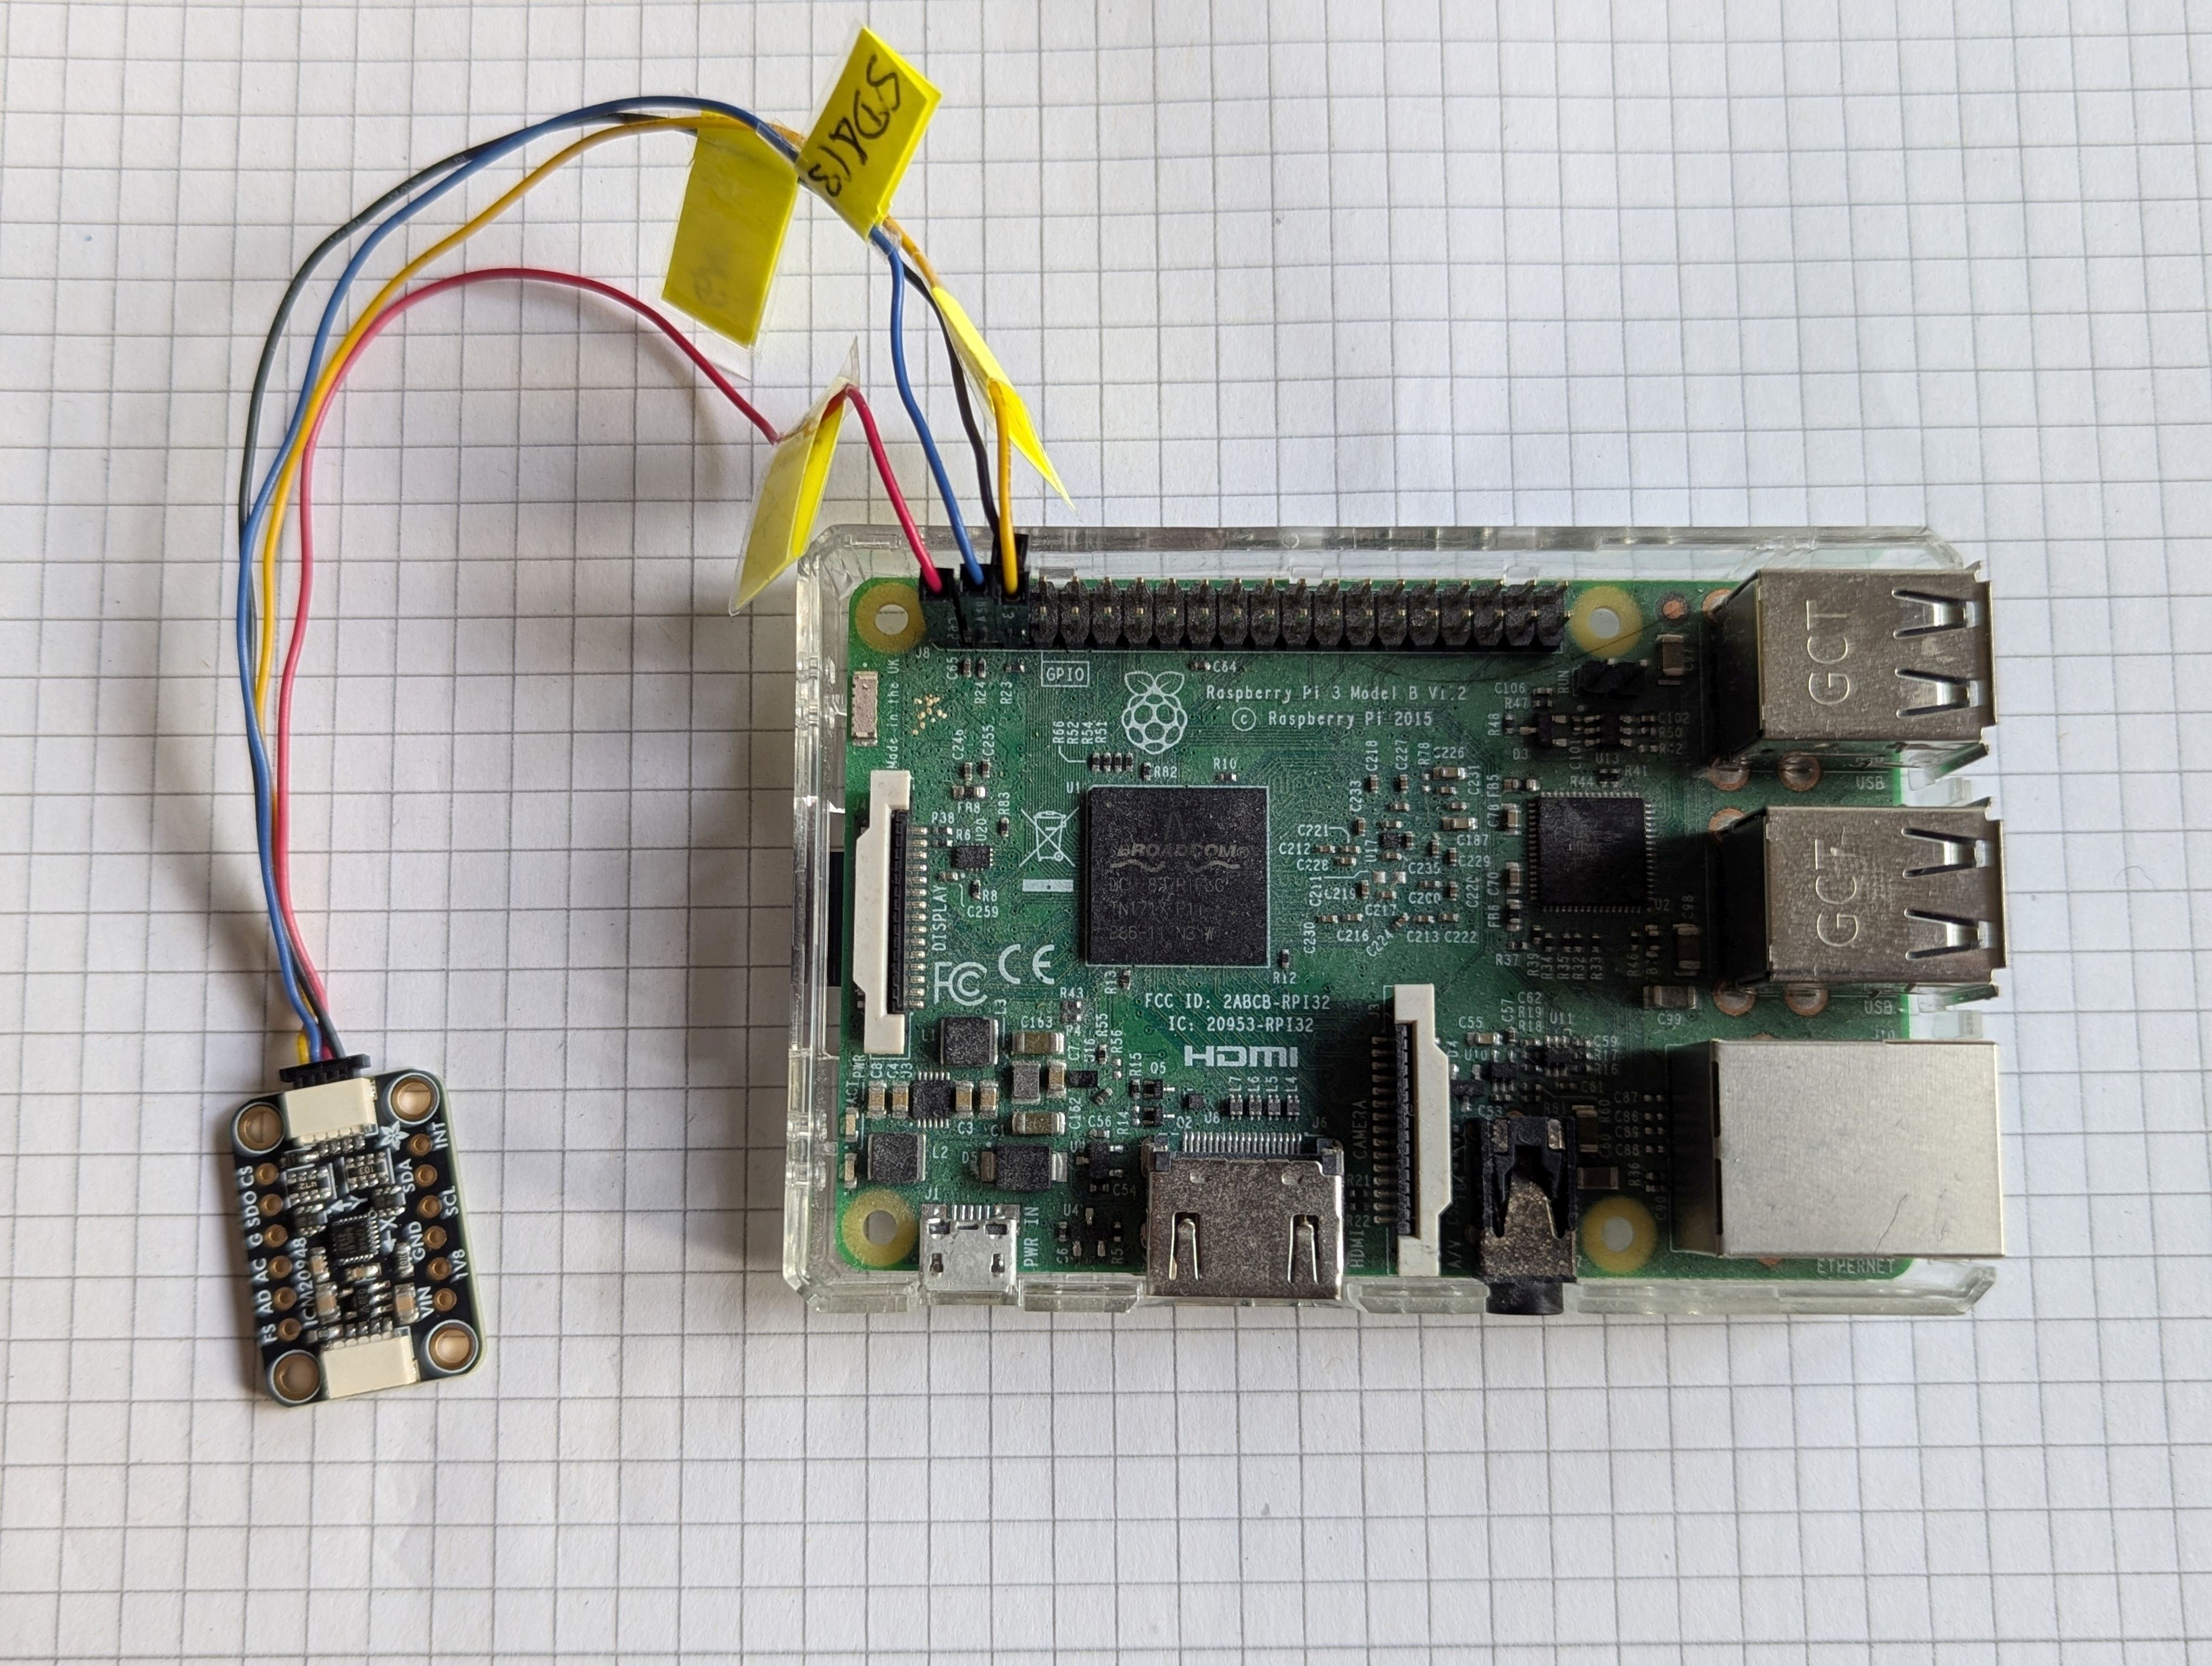
\includegraphics[width=12cm]{images/rpi3_with_icm20948.jpg}
	\caption{Raspberry Pi 3 with ICM20948}
\end{figure}	


\section{Programming the ICM20948 with Python}

To access the I2C bus programmatically from Python at least the \verb|smbus2| library needs to be installed. The library defines a class \verb|SMBus| with methods for reading / writing to a I2C device.

The documentation of the library is available at \url{https://smbus2.readthedocs.io/en/latest}.

To see whether the ICM20948 sensor can be accessed a test is done directly in the Python shell of the Raspberry Pi. Here is an interactive session which reads out the chip id of the ICM20948.

\begin{verbatim}
	mbi1955@raspberrypi:~ $ python3
	Python 3.9.2 (default, Mar 20 2025, 22:21:41)
	[GCC 10.2.1 20210110] on linux
	Type "help", "copyright", "credits" or "license" for more information.
	>>> from smbus2 import SMBus
	>>> ic2bus = SMBus(1)
	>>> I2C_ADDR = 0x69
	>>> WHO_AM_I = 0x00
	>>> BANK_SEL = 0x7f
	>>> bank = 0
	>>> ic2bus.write_byte_data(I2C_ADDR, BANK_SEL, bank)
	>>> chip_id = ic2bus.read_byte_data(I2C_ADDR, WHO_AM_I)
	>>> print(f"who_am_i: {hex(chip_id)}")
	who_am_i: 0xea
\end{verbatim}

Not surprisingly the output \verb|0xea| is identical to what we got using Linux command   \verb|i2cget|.

For a more convenient working environment another library seems to be useful. 

Library \url{https://pypi.org/project/icm20948/} defines some methods which make working with the ICM20948 a bit easier. It defines some constants and addresses along with a Python class \verb|ICM20948| which has methods for initialisation and reading/writing .

Before trying to understand some details how the sensor is initially configured, the usage of the library shall be tested with a Python program.

\begin{verbatim}
# icm20948_test.py

from icm20948 import *
import time

if __name__ == "__main__":
imu = ICM20948(i2c_addr=I2C_ADDR_ALT, i2c_bus=None)

for k in range(3):
x, y, z = imu.read_magnetometer_data()
ax, ay, az, gx, gy, gz = imu.read_accelerometer_gyro_data()

print(f"""
Accel: {ax:05.2f} {ay:05.2f} {az:05.2f}
Gyro:  {gx:05.2f} {gy:05.2f} {gz:05.2f}
Mag:   {x:05.2f} {y:05.2f} {z:05.2f}""")

time.sleep(0.25)
\end{verbatim}

And the output is:

\begin{verbatim}
mbi1955@raspberrypi:~/Projects/icm20948 $ /usr/bin/python3 /home/mbi1955/Projects/icm20948/icm20948_test.py

Accel: -0.13 -0.33 00.96
Gyro:  -1.34 00.27 00.02
Mag:   -38.10 -67.05 74.10

Accel: -0.13 -0.33 00.95
Gyro:  -1.19 00.25 00.05
Mag:   -38.10 -67.05 74.40

Accel: -0.14 -0.33 00.95
Gyro:  -1.32 00.14 00.15
Mag:   -37.20 -67.20 73.20
\end{verbatim}

The output shows that reading out the 3-axis values of

\begin{compactitem}
	\item accelerometer
	\item gyroscope
	\item magnetometer
\end{compactitem}

works in principle. Three readings have been obtained with a time interval between readings of 0.25 seconds. Between the measurements the sensor has not been moved. Accordingly the values are more or less constant (apart from measurement noise).

Now that we have confirmed the functionality of library \verb|icm20948| we shall look into the details of configuring the accelerometer, gyroscope and magnetometer. The library provides several methods to accomplish initial configuration tasks.

\subsection{resetting the ICM20948}

The MSB (Bit 7) of register \verb|PWR_MGMT_1| is set.

Bits 2:0 of register \verb|PWR_MGMT_1| are set to 1. The data sheet states: 1-5: Auto selects the best available clock source – PLL if ready, else use the Internal oscillator.

Register \verb|PWR_MGMT_2| is set to \verb|0x00|. All axes of accelerometer and gyroscope are turned on.


\subsection{accelerometer / initial configuration}

The initial configuration comprises settings of the sampling rate, low pass filter, the scale/range of accelerometer.

\subsubsection{samplerate}

The samplerate can be configured in the range 4.5 to 1125 Hz. The actual sampling rate $f_s$ is computed using this equation:

\[
f_s = \frac{1125~Hz}{1 + ratio}
\]

where $ratio$ is a 12 bit number configured via registers \verb|ACCEL_SMPLRT_DIV_1| and \verb|ACCEL_SMPLRT_DIV_2|.


Example: to configure a sampling rate of $f_s = 125~Hz$ we must choose $ratio = 8$.

\subsubsection{low pass filter}

The low pass filter is enabled setting the LSB of register \verb|ACCEL_CONFIG| to 1.

The bandwidth of the low pass filter is then configured via bits 5:3 of the same register.

\subsubsection{full scale}

Bits 2:1 of \verb|ACCEL_CONFIG| configure the scale (min/max range) of the accelerometer. 

\subsection{gyroscope / initial configuration}

\subsubsection{samplerate}

The samplerate can be configured in the range 4.5 to 1125 Hz. The actual sampling rate $f_s$ is computed using this equation:

\[
f_s = \frac{1125~Hz}{1 + ratio}
\]

where $ratio$ is a 8 bit number configured via registers \verb|GYRO_SMPLRT_DIV|.

Example: to configure a sampling rate of $f_s = 125~Hz$ we must choose $ratio = 8$.

\subsubsection{low pass filter}

The low pass filter is enabled setting the LSB of register \verb|GYRO_CONFIG_1| to 1.

The bandwidth of the low pass filter is then configured via bits 5:3 of the same register.

\subsubsection{full scale}

Bits 2:1 of \verb|GYRO_CONFIG_1| configure the scale (min/max range) of the accelerometer. 

\subsection{magnetometer / initial configuration}

The magnetometer is reset 

\section{Exploring the accelerometer and the gyroscope}

A sample Python program has been written which records a user defined number of samples of the (x,y,z)-data of the accelerometer and the gyroscope. The data are stored in as compressed Numpy file.

The ICM20948 sensor is oriented in various static positions. For each position the recorded data are stored in a file.

A \texttt{Jupyter} notebook retrieves data from these files and produces some graphics to illustrate how accelerometer and gyroscope data behave under static, arbitrary but fixed orientation.

The static recordings indicate that for any meaningful application the accelerometer must be calibrated to compensate for a number of non-ideal properties:

\begin{compactitem}
	\item misalignment of x,y,z sensors (not being exactly mutually orthogonal)
	\item sensitivity error; scaling factors in x,y,z direction are not identical
	\item additive offsets
\end{compactitem}

Another test for the gyroscope shows that readings will benefit from calibration as well. The sensors of the gyroscope have significant offsets. An example in the notebook shows, that angle data obtained from postprocessing raw gyroscope data exhibit a large drift over time if these offsets are not compensated for.




	
\end{document}
